%%
%% Author: thompson
%% 25.12.17
%%

% Preamble
\documentclass[11pt]{article}

% Packages
\usepackage{a4wide}
\usepackage[utf8]{inputenc}
\usepackage[naustrian]{babel}

\usepackage{enumerate}
\usepackage{verbatim}
\usepackage{scrextend}
\usepackage{graphicx}

\title{Rechnernetze - Übungsblatt 9}
\author{Auer Thomas}    % Add if u did add
\date{WS17}

% Document
\begin{document}
    \section{TCP - Transfer Control Protocol}
    \subsection{TCP Philosophie}
    Wenden Sie Ihr Wissen aus der Vorlesung an und beantworten Sie folgende Fragen:
    \begin{enumerate}[$\bullet$]
        \item Wie wird eine Verbindung beim TCP-Protokoll aufgebaut?\\
        Mittels Kontrollpaketen wird zunächst Kontakt zum Serverhost aufgenommen.
        Im sog. 'Handshake' wird anschließend Kontaktinformation ausgetauscht, die notwendig sind um Datenpackete zu
        senden und zu empfangen.

        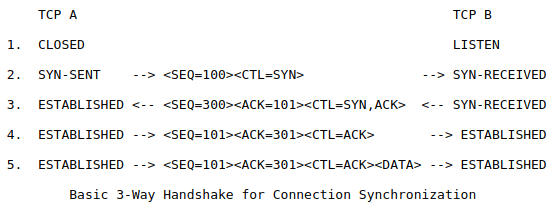
\includegraphics[width=\textwidth]{graphics/TCPHandshake.png}

        \item Wie wird eine Verbindung beim TCP-Protokoll abgebaut?\\
        Der Verbindungsabbau wird mittels der FIN-Flag initiiert. Sobald der Klient diese Kontrollinformation sendet,
        darf dieser keine Informationen mehr senden, jedoch weiterhin empfangen.
        Nach einem Timeout oder nach Empfang des gesetzten Flag-Bits des Servers wird die Verbindung terminiert.

        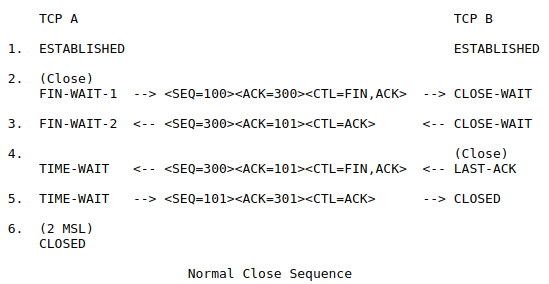
\includegraphics[width=\textwidth]{graphics/TCPClose.png}

        \item Können bei der Übertragung durch das TCP-Protokoll TCP-Segmente verloren gehen? Wenn ja: Was
        passiert dann?\\
        Die SEQ und ACK-Werte helfen bei der Identifikation eventuell verloren gegangener Packete. Im Falle dessen wird
        einfach das jeweilige Packet erneut gesendet.

        \item Wie werden die Sequenznummern lt. RFC vergeben?\\
        Die Sequenznummern werden nach striktem Muster vergeben, mithilfe der ACK.
        Die allererste SEQ-Nummer wird zufällig gewählt. Beim Datenempfang wird diese Nummer extrahiert und als ACK-Wert
        gesetzt. Der zurückgesendete SEQ-Wert hat den Wert der alten ACK + Payload derselben Nachricht.
        Dies tauscht sich fotwährend nach diesem Schema ab.
    \end{enumerate}

    \subsection{TCP Spezifikationen}
    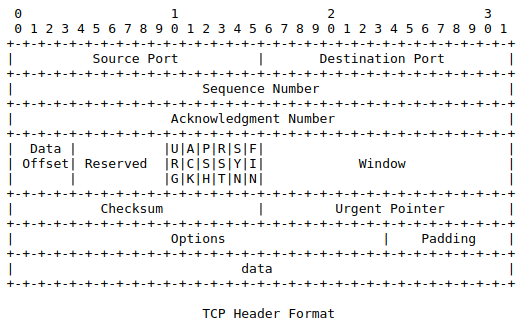
\includegraphics[width=\textwidth]{graphics/TCPStruct.png}
    \begin{addmargin}[1em]{1em}
        $\bullet$ Source Port: Port des Senders\\
        $\bullet$ Destination Port: Port des Empfängers\\
        $\bullet$ SEQNummer: Wenn SYN gesetzt, so ist es ISN + 1; Andernfalls First data Octet in Segment\\
        $\bullet$ ACKNummer: Bestätigt SEQ\\
        $\bullet$ Data Offset: Indiziert Datenbeginn\\
        $\bullet$ Reserved: Must be Zero\\
        $\bullet$ Controlbits:
        \begin{addmargin}[1em]{1em}
            $\circ$ URG: Urgent Pointer, Abhängig von Feld\\
            $\circ$ ACK: Acknowledgment, Abhängig vom Feld\\
            $\circ$ PSH: Push Funktion\\
            $\circ$ RST: Reset Connection\\
            $\circ$ SYN: Synchronize for first connection establishment\\
            $\circ$ FIN: No more data from sender, close the connection
        \end{addmargin}
        $\bullet$ Window: Anzahl der Datenoktets welche vom Sender angenommen werden.\\
        $\bullet$ Checksum: Validiert Datenpacket.\\
        $\bullet$ Options: Variiert. Inkludiert alle Optionen, derzeit:
    \end{addmargin}
    \begin{verbatim}
    0.EOL       1.No-Operation    2.Maximum Segment Size
    +--------+    +--------+      +--------+--------+--------+--------+
    |00000000|    |00000001|      |00000010|00000100|   max seg size  |
    +--------+    +--------+      +--------+--------+--------+--------+
    \end{verbatim}
    \begin{addmargin}[1em]{1em}
        $\bullet$ Maximum Segment Size Option Data - Maximum Size of TCP-Packet size. Set in the initial connection request.\\
        $\bullet$ Padding: Variable, Composed of 0'.
    \end{addmargin}

    \subsection{TCP Eigenschaften}
        $\diamond$ Full Duplex - Bidirektionaler Datenfluss\\
        $\diamond$ Verbindungsorientiert - Verbindungsaufbau vor Datenaustausch; Point-to-Point\\
        $\diamond$ Flow control - Datenspeicherung im Empfangsbuffer läuft über -- Empfänger steuert Transfer via Angaben\\
        $\diamond$ Congestion control - Packetoverflow im Subnet -- Zuviele Quellen schicken zuviele Daten, Datenverwurf auf Netzwerkschicht/IP-Layer.\\
        $\diamond$ In-order byte stream - Präventionen für Datenverlust \& Datenempfang\\
        $\diamond$ Pipelined: Multiple Datenübertragungen: Selective Repeat, Go-Back-N,...\\
\end{document}

